\section{Additional Details}
\label{app:details}

\para{Per-model accuracy.}
\Figref{fig:acc_app} visualizes the accuracies in \tabref{tab:accuracy}.

\begin{figure}[ht]
    \centering
    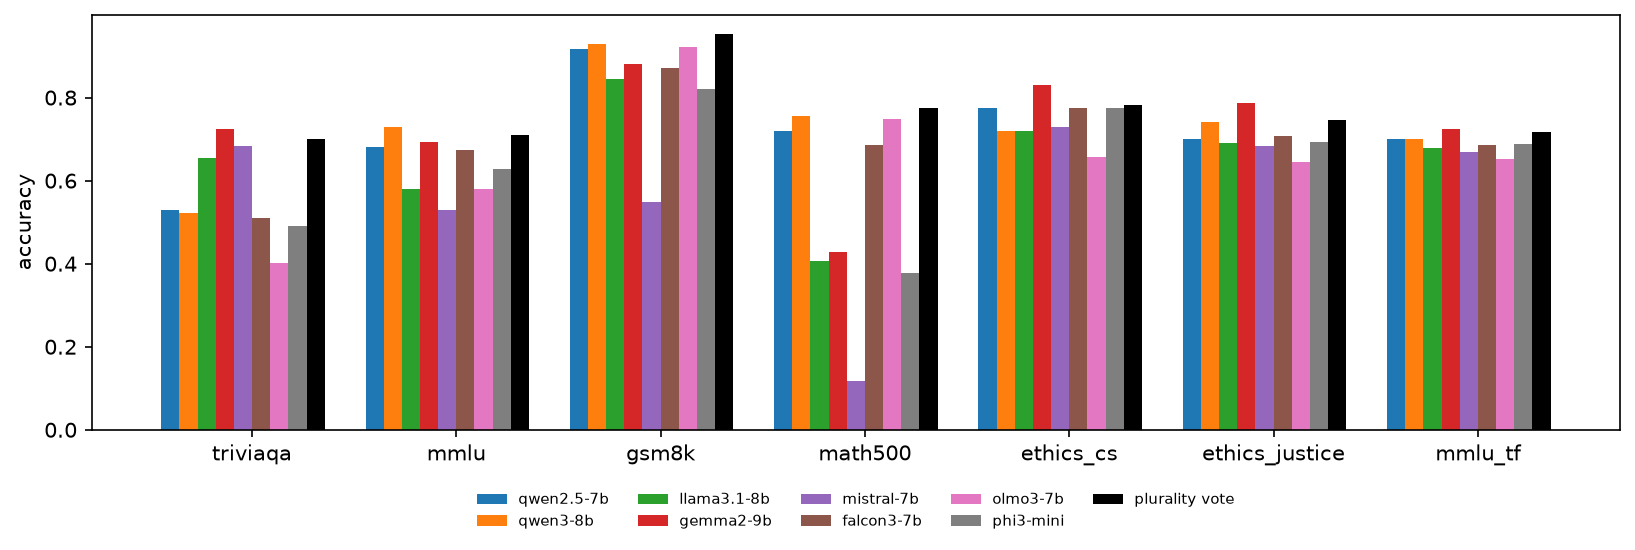
\includegraphics[width=0.9\linewidth]{figures/accuracy_models_vs_vote.png}
    \caption{Accuracy of each model and of the 8-model plurality vote on each task.}
    \label{fig:acc_app}
\end{figure}

\para{Selective prediction at two thresholds.}
\Tabref{tab:selective_app} lists coverage and accuracy when the system answers only items with agreement at or above a threshold.

\begin{table}[ht]
    \centering
    \small
    \begin{tabular}{@{}lccccc@{}}
        \toprule
        & & \multicolumn{2}{c}{$a(x) \geq 0.75$} & \multicolumn{2}{c}{$a(x) = 1$} \\
        \cmidrule(lr){3-4} \cmidrule(lr){5-6}
        \textbf{Dataset} & Acc.\ (all) & Coverage & Accuracy & Coverage & Accuracy \\
        \midrule
        \triviaqa & 0.701 & 0.369 & 0.939 & 0.143 & 0.957 \\
        \mmlu     & 0.710 & 0.604 & 0.868 & 0.274 & 0.971 \\
        \gsm      & 0.952 & 0.854 & 0.984 & 0.450 & 0.991 \\
        \mathfive & 0.776 & 0.374 & 0.989 & 0.066 & 1.000 \\
        \ethcs    & 0.782 & 0.810 & 0.830 & 0.494 & 0.903 \\
        \ethjus   & 0.746 & 0.850 & 0.772 & 0.468 & 0.833 \\
        \mmlutf   & 0.718 & 0.688 & 0.805 & 0.304 & 0.934 \\
        \bottomrule
    \end{tabular}
    \caption{Selective prediction using inter-model agreement as the abstention rule.}
    \label{tab:selective_app}
\end{table}

\para{One model per family.}
\Tabref{tab:family_app} repeats the main analysis without qwen3-8b, so that each developer family contributes one model (7 models).

\begin{table}[ht]
    \centering
    \small
    \begin{tabular}{@{}llcccc@{}}
        \toprule
        \textbf{Dataset} & \textbf{Best model} & Vote acc. & Vote $-$ best (pp) & $r$ & AUROC \\
        \midrule
        \triviaqa & gemma2-9b (0.725) & 0.709 & $-1.6$ & 0.538 & 0.841 \\
        \mmlu     & gemma2-9b (0.692) & 0.686 & $-0.6$ & 0.462 & 0.784 \\
        \gsm      & olmo3-7b (0.922)  & 0.940 & $+1.8$ & 0.438 & 0.869 \\
        \mathfive & olmo3-7b (0.748)  & 0.752 & $+0.4$ & 0.587 & 0.891 \\
        \ethcs    & gemma2-9b (0.830) & 0.788 & $-4.2$ & 0.321 & 0.711 \\
        \ethjus   & gemma2-9b (0.788) & 0.734 & $-5.4$ & 0.223 & 0.640 \\
        \mmlutf   & gemma2-9b (0.724) & 0.714 & $-1.0$ & 0.366 & 0.727 \\
        \bottomrule
    \end{tabular}
    \caption{Results with one model per family. The conclusions match the full pool.}
    \label{tab:family_app}
\end{table}

\para{Implementation.}
We used vLLM 0.31.0 with a maximum context length of 2,560 tokens.
A scheduler waited for free GPU memory and retried runs that failed at startup.
Every rendered prompt, all raw generations and all parsed answers are stored with the code.
The API cost was zero.
